
% !TEX encoding = UTF-8 Unicode 
% !TEX root = FieldGuide.tex

\clearpage
\thispagestyle{chapter}
\begin{figure*}
\phantomsection\addcontentsline{toc}{section}{Distribution hierarchies} 
\phantomsection\addcontentsline{toc}{subsection}{Hierarchy of principal distributions} 
\caption[Hierarchy of principal distributions]{Hierarchy of principal distributions} 
\label{PrincipalHierarchy}
\begin{center}
\scalebox{0.58} {
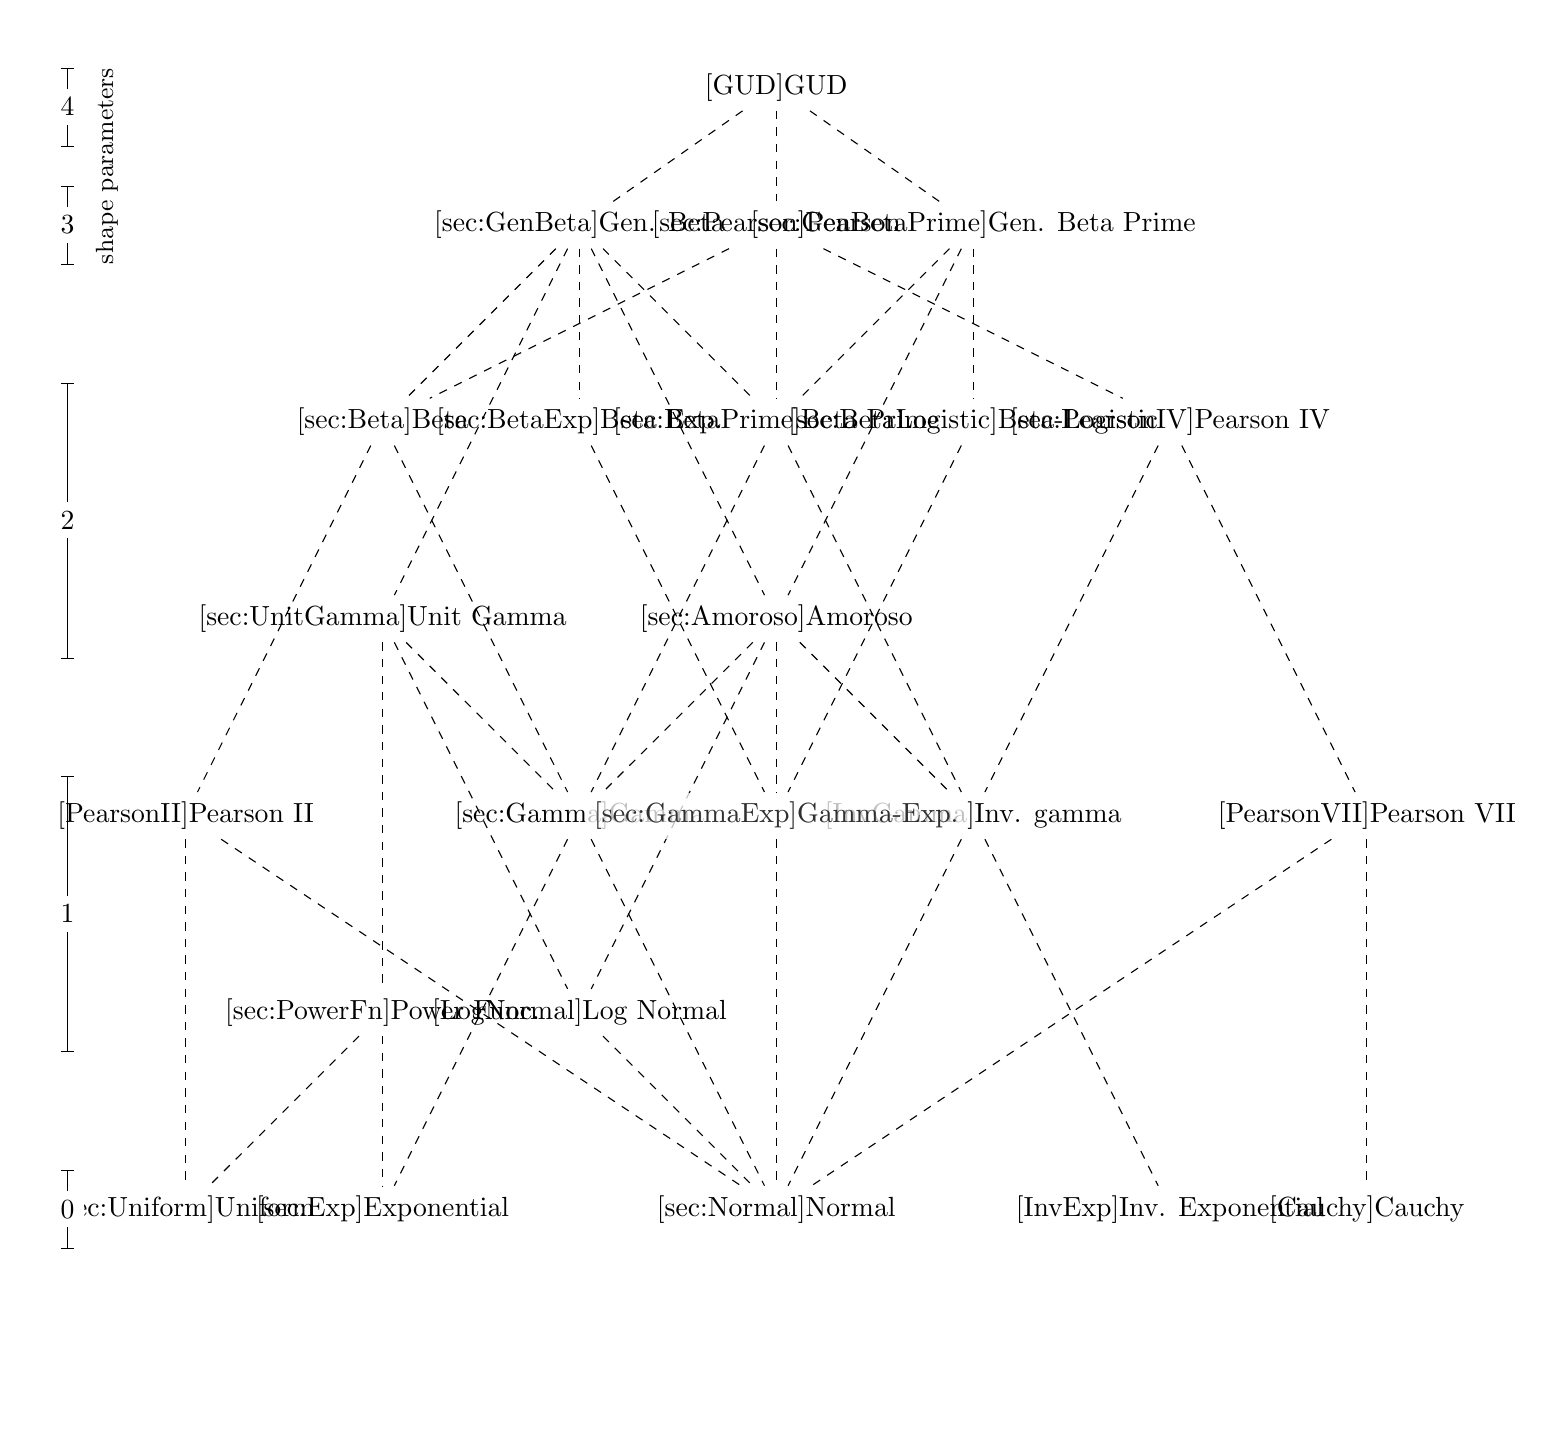
\begin{tikzpicture}
%\draw[help lines, very thin, step=1] (-2,0) grid (17,17);
%
\draw (7.5,16.75) node (gud) {\hyperref[GUD]{GUD}};
%
\draw (5,15) node (genbeta) {\hyperref[sec:GenBeta]{Gen. Beta}};
\draw (7.5,15) node (pearson) {\hyperref[sec:Pearson]{Pearson}};
\draw (10,15) node (genbetaprime) {\hyperref[sec:GenBetaPrime]{Gen. Beta Prime}};
%
\draw (2.5,12.5) node (beta) {\hyperref[sec:Beta]{Beta}};
\draw (5,12.5) node (betaexp) {\hyperref[sec:BetaExp]{Beta Exp.}};
\draw (7.5,12.5) node (betaprime) {\hyperref[sec:BetaPrime]{Beta Prime}};
\draw (10,12.5) node (betalogistic) {\hyperref[sec:BetaLogistic]{Beta-Logistic}};
\draw (12.5,12.5) node (pearsoniv) {\hyperref[sec:PearsonIV]{Pearson IV}};
%
\draw (2.5,10) node (unitgamma) {\hyperref[sec:UnitGamma]{Unit Gamma}};
\draw (7.5,10) node (amoroso) {\hyperref[sec:Amoroso]{Amoroso}};
%\draw (12.5,10) node (burr) {\hyperref[Burr]{Burr}};
%
\draw (0,7.5) node  (pearsonii) {\hyperref[PearsonII]{Pearson II}};
\draw (2.5,5) node (power)  {\hyperref[sec:PowerFn]{Power Func.}};
\draw (5,7.5) node  (gamma) {\hyperref[sec:Gamma]{Gamma}};
\draw (7.5,7.5) node (gammaexp)  {\hyperref[sec:GammaExp]{Gamma-Exp.}};
\draw (10,7.5) node (invgamma) {\hyperref[InvGamma]{Inv. gamma}}; 
%\draw (12.5,7.5) node  (loglogistic) {\hyperref[LogLogistic]{Log-Logistic}};
\draw (15,7.5) node (pearsonvii) {\hyperref[PearsonVII]{Pearson VII }};
%
%\draw (5,5) node (weibull) {\hyperref[Weibull]{Weibull}};
%\draw (7.5,5) node (symbetalogistic) {\hyperref[SymBetaLogistic]{Sym. Beta-Logistic}};
%\draw (10,5) node (frechet) {\hyperref[Frechet]{Frechet}};
%\draw (12.5,7.5) node (lognormal) {\hyperref[LogNormal]{Log Normal}};
\draw (5,5) node (lognormal) {\hyperref[LogNormal]{Log Normal}};
%
\draw (0,2.5) node (uniform) {\hyperref[sec:Uniform]{Uniform}};
\draw (2.5,2.5) node (exp) {\hyperref[sec:Exp]{Exponential}};
%\draw (5,2.5) node (laplace) {\hyperref[sec:Laplace]{Laplace}};
\draw (7.5,2.5) node (normal) {\hyperref[sec:Normal]{Normal}};
%\draw (10,2.5) node (UniPrime) {\hyperref[Logistic]{Uniform Prime}};
%\draw (10,2.5) node (logistic) {\hyperref[Logistic]{Logistic}};
\draw (12.5,2.5) node (invexp) {\hyperref[InvExp]{Inv. Exponential}};
\draw (15,2.5) node (cauchy) {\hyperref[Cauchy]{Cauchy}};
%
%\draw (7.5,0) node (gumbel) {\hyperref[Gumbel]{Gumbel}};
%
\draw [dashed]  (gud) -- (genbeta);
\draw [dashed]  (gud) -- (pearson);
\draw [dashed]  (gud) -- (genbetaprime);
%
\def\betaone{node}%
\draw [dashed]  (genbeta) --  (beta);
\draw [dashed]  (genbeta) --  (betaexp);
\draw [dashed]  (genbeta) --  (betaprime);
\draw [dashed]  (genbeta) -- (unitgamma);
\draw [dashed]  (genbeta) -- (amoroso);
%
\draw [dashed]  (pearson) -- (beta);
\draw [dashed]  (pearson) -- (betaprime);
\draw [dashed]  (pearson) -- (pearsoniv);
%
\draw [dashed]  (genbetaprime) -- (betalogistic);
\draw [dashed]  (genbetaprime) -- (betaprime);
\draw [dashed]  (genbetaprime) -- (amoroso);
%\draw [dashed]  (genbetaprime) -- (burr);
%
\draw [dashed]  (beta) -- (pearsonii);
\draw [dashed]  (beta) -- (gamma);
%
\draw [dashed]  (betaexp) -- (gammaexp);
%
\draw [dashed]  (betaprime) -- (gamma);
\draw [dashed]  (betaprime) -- (invgamma);
%
\draw [dashed]  (betalogistic) -- (gammaexp);
%\draw [dashed]  (betalogistic) -- (symbetalogistic);
%
\draw [dashed]  (pearsoniv) -- (invgamma);
\draw [dashed]  (pearsoniv) -- (pearsonvii);
\draw [dashed] (unitgamma) -- (power);
\draw [dashed]  (unitgamma) -- (gamma);
%
\draw [dashed]  (amoroso) -- (gamma);
%\draw [dashed]  (amoroso) -- (weibull);
\draw [dashed]  (amoroso) -- (gammaexp);
\draw [dashed]  (amoroso) -- (invgamma);
%\draw [dashed]  (amoroso) -- (frechet);
%
%\draw [dashed]  (burr) -- (frechet);
%\draw [dashed]  (burr) -- (loglogistic);
%
\draw [dashed]  (pearsonii) -- (uniform);
\draw [dashed]  (pearsonii) -- (normal);
\draw [dashed]  (power) -- (uniform);
\draw [dashed]  (power) -- (exp);
\draw [dashed]  (gamma) -- (exp);
\draw [dashed]  (gamma) -- (normal);
\draw [dashed]  (invgamma) -- (normal);
\draw [dashed]  (invgamma) -- (invexp);
%\draw [dashed]  (loglogistic) -- (logistic);
\draw [dashed]  (pearsonvii) -- (normal);
\draw [dashed]  (pearsonvii) -- (cauchy);
%
%\draw [dashed]  (weibull) -- (exp);
%\draw [dashed]  (weibull) -- (gumbel);
%\draw [dashed]  (symbetalogistic) -- (laplace);
%\draw [dashed]  (symbetalogistic) -- (normal);
%\draw [dashed]  (symbetalogistic) -- (logistic);
%\draw [dashed]  (frechet) -- (gumbel);
%\draw [dashed]  (frechet) -- (invexp);
\draw [dashed] (amoroso) -- (lognormal);
\draw [dashed] (unitgamma) -- (lognormal);		
\draw [dashed] (lognormal) -- (normal);
%
%\draw [dashed] (amoroso) -- +(5, -1.5)-- (lognormal);
%\draw [dashed] (gammaexp) -- +(0,-1) ;
%\draw [dashed] (gumbel) -- +(0,0.75) ;
%\draw [dashed] (gammaexp)  -- (gumbel) ;
\draw [dashed] (gammaexp)  -- (normal) ;
%
\draw (7.5,7.5) node[fill=white, fill opacity=0.75] {\hyperref[sec:GammaExp]{Gamma-Exp.}};
%\draw (7.5,5) node[fill=white, fill opacity=0.75] {\hyperref[SymBetaLogistic]{Sym. Beta-Logistic}};
%
\draw[|-|, very thin] (-1.5,2) -- node[fill=white, midway] {0} (-1.5,3);
\draw[|-|, very thin]  (-1.5,4.5) -- node[fill=white, midway] {1} (-1.5,8);
\draw[|-|, very thin]  (-1.5,9.5) -- node[fill=white, midway] {2} (-1.5,13);
\draw[|-|, very thin]  (-1.5,14.5) -- node[fill=white, midway] {3} (-1.5,15.5);
\draw[|-|, very thin]  (-1.5,16) -- node[fill=white, midway] {4} (-1.5,17);
%
\draw (-1, 15.75) node[rotate=90]  {\small shape parameters};
%
\draw[white] (-2, 0) rectangle (17,17.5); % Bounding box
\end{tikzpicture}
}
\end{center}
\end{figure*}

